%%
%% Copyright 2007, 2008, 2009 Elsevier Ltd
%%
%% This file is part of the 'Elsarticle Bundle'.
%% ---------------------------------------------
%%
%% It may be distributed under the conditions of the LaTeX Project Public
%% License, either version 1.2 of this license or (at your option) any
%% later version.  The latest version of this license is in
%%    http://www.latex-project.org/lppl.txt
%% and version 1.2 or later is part of all distributions of LaTeX
%% version 1999/12/01 or later.
%%
%% The list of all files belonging to the 'Elsarticle Bundle' is
%% given in the file `manifest.txt'.
%%

%% Template article for Elsevier's document class `elsarticle'
%% with harvard style bibliographic references
%% SP 2008/03/01
%%
%%
%%
%% $Id: elsarticle-template-harv.tex 4 2009-10-24 08:22:58Z rishi $
%%
%%
%% \documentclass[preprint,authoryear,12pt]{elsarticle}

%% Use the option review to obtain double line spacing
%% \documentclass[authoryear,preprint,review,12pt]{elsarticle}

%% Use the options 1p,twocolumn; 3p; 3p,twocolumn; 5p; or 5p,twocolumn
%% for a journal layout:
%% \documentclass[final,authoryear,1p,times]{elsarticle}
%% \documentclass[final,authoryear,1p,times,twocolumn]{elsarticle}
%% \documentclass[final,authoryear,3p,times]{elsarticle}
\documentclass[final,authoryear,3p,times,twocolumn]{elsarticle}
%% \documentclass[final,authoryear,5p,times]{elsarticle}
%% \documentclass[final,authoryear,5p,times,twocolumn]{elsarticle}

%%-------------------------------------------------------------------------------
%add ukrainian locale
\usepackage[ukrainian,russian,english]{babel}
\usepackage[utf8]{inputenc}
\usepackage[T2A]{fontenc}
%mathematical symbols
\usepackage{gensymb}
%%-------------------------------------------------------------------------------


%% if you use PostScript figures in your article
%% use the graphics package for simple commands
%% \usepackage{graphics}
%% or use the graphicx package for more complicated commands
\usepackage{graphicx}
%% or use the epsfig package if you prefer to use the old commands
\usepackage{epsfig}

%% The amssymb package provides various useful mathematical symbols
\usepackage{amssymb}
%% The amsthm package provides extended theorem environments
%% \usepackage{amsthm}

%% The lineno packages adds line numbers. Start line numbering with
%% \begin{linenumbers}, end it with \end{linenumbers}. Or switch it on
%% for the whole article with \linenumbers after \end{frontmatter}.
%% \usepackage{lineno}

%% for sub[super]script
\usepackage{fixltx2e}

%% natbib.sty is loaded by default. However, natbib options can be
%% provided with \biboptions{...} command. Following options are
%% valid:

%%   round  -  round parentheses are used (default)
%%   square -  square brackets are used   [option]
%%   curly  -  curly braces are used      {option}
%%   angle  -  angle brackets are used    <option>
%%   semicolon  -  multiple citations separated by semi-colon (default)
%%   colon  - same as semicolon, an earlier confusion
%%   comma  -  separated by comma
%%   authoryear - selects author-year citations (default)
%%   numbers-  selects numerical citations
%%   super  -  numerical citations as superscripts
%%   sort   -  sorts multiple citations according to order in ref. list
%%   sort&compress   -  like sort, but also compresses numerical citations
%%   compress - compresses without sorting
%%   longnamesfirst  -  makes first citation full author list
%%
\bibliographystyle{ieeetr}
\biboptions{numbers,square}

%% \biboptions{}

\journal{Physica B}

\begin{document}

\begin{frontmatter}

%% Title, authors and addresses

%% use the tnoteref command within \title for footnotes;
%% use the tnotetext command for the associated footnote;
%% use the fnref command within \author or \address for footnotes;
%% use the fntext command for the associated footnote;
%% use the corref command within \author for corresponding author footnotes;
%% use the cortext command for the associated footnote;
%% use the ead command for the email address,
%% and the form \ead[url] for the home page:
%%

\title{{\LARGE An EPR studies of V\textsubscript{C}C\textsubscript{Si}\textsuperscript{-} defect in neutron irradiated 3C-SiC}}
%% \tnotetext[label1]{}
\author[dep]{V. Bratus'\corref{cor1}}
\ead{v\_bratus@isp.kiev.ua}

\author[dep]{R. Melnyk\corref{cor2}}
\ead{melnyk\_rs@yahoo.com}

\author[dep]{S. Okulov}
\author[lab]{V. Strelchuk}
\author[lab]{O. Kolomys}

\cortext[cor1]{Corresponding author. Tel.: +380-44-265-8560}
\cortext[cor2]{Corresponding author. Tel.: +380-93-146-8353}
\address[dep]{\small Department of Optics and Spectroscopy, V. Lashkaryov Institute of Semiconductor Physics, National Academy of Sciences of Ukraine, 45 pr. Nauky, 03680 Kyiv, Ukraine}
\address[lab]{\small Raman Laboratory at V. Lashkaryov Institute of Semiconductor Physics, National Academy of Sciences of Ukraine, 45 pr. Nauky, 03680 Kyiv, Ukraine}

%% \title{}

%% use optional labels to link authors explicitly to addresses:
%% \author[label1,label2]{<author name>}
%% \address[label1]{<address>}
%% \address[label2]{<address>}

\author{}

\address{}

\begin{abstract}
  Annealing the n-type neutron-irradiated 3C-SiC crystals at T~=~900~\degree C leads to full vanishing of silicon vacancies and simultaneous emergence of new paramagnetic defect, called Ky6. New center has spin S~=~1/2 and can be described with axial g-factor directed along <111> direction and with principal parameters g$_\parallel$~=~2.0024 and g$_\perp$~=~2.0029. Ky6 center can be observed at temperatures under 140 K and shows hyperfine interaction (HF) with principal parameters А$_\parallel$~=~23.9$\cdot$10$^{-4}$~cm$^{-1}$ and А$_\perp$~=~19.3$\cdot$10$^{-4}$~cm$^{-1}$. Based on the HF parameters, annealing processes of defects in crystal and calculations of formation energies \citep{met1,met2} center Ky6 was tentatively assigned to V\textsubscript{C}C\textsubscript{Si}\textsuperscript{0} in 3C-SiC.

\end{abstract}


\begin{keyword}
%% keywords here, in the form: keyword \sep keyword
3C-SiC\sep EPR\sep Intrinsic defect\sep Thermal annealing

%% MSC codes here, in the form: \MSC code \sep code
%% or \MSC[2008] code \sep code (2000 is the default)

\end{keyword}
% \linenumbers

\end{frontmatter}

%% main text
\section{Introduction}Due to its remarkable electronic and physical properties, silicon carbide takes a substantial place among all semiconducting materials. High thermal, radiational and chemical endurance makes it a significant substance for developing electronic devices that can be used in severe environments like space or nuclear reactors.\\
\indent There are over 200 polytypes of SiC, but cubic 3C-SiC has simplest crystal structure and highest electron mobility among all \citep{choy1}. Unfortunately, due to complexity in growth conditions of 3C-SiC it has not reached vast industrial implementation. Simultaneously the greater commercial success have been reached for hexagonal crystals and therefore they much better studied during past decades (see \citep{hex1, hex2} and references therein). However, recent progress in 3C-SiC growth, especially thin films \citep{epilay}, raised up interest for industrial use of cubic crystals as basis for industrial electronics.\\
\indent Irradiation of crystal produces high concentrations of various point defects and therefore influences on its electronic properties. Thus perspectives of industrial use of 3C-SiC raises the interest to studying properties of its point defects. Dominant defects in as-irradiated 3C-SiC crystals are negative silicon vacancy \citep{t1} and neutral divacancy \citep{ky5}. Silicon vacancy was observed in crystals irradiated by electrons, protons, neutrons and ions, has spin S~=~3/2 and can be described by isotrop g~=~2.0029. From another hand, divacancy observed only in neutron irradiated samples, has S~=~1 and axial fine structure tensor and isotrop g-factor: D~=~443$\cdot10^{-4}$ cm$^{-1}$ and g~=~2.003 respectively. Annealing at Т\textsubscript{ann}~=~900~K cause transformations in system of defects that results in almost full disappearence of mentioned above defects. At the same time, new EPR spectrum was emerging. This spectrum was linked to S~=~1/2 paramagnetic defect, named Ky6, and the present paper has been dedicated for elucidate properties of this defect.
 
%% \label{}
\section{Experimental}All samples were grown by vapor-phase process.  Thermal decomposition of methyl trichlorsilane in hydrogen environment at T~=~1700~K and consequent precipitation on graphite needles used to obtain required compound during this process. All samples weren't intentionaly doped and n-type of conductivity had been set by Nitrogen donors, that formed during crystal growth. Concentration of this donors were 10$^{17}$~cm$^{-3}$. Typical sample dimentions were 4~x~3~x~0.7 mm. Neutron irradiation were carried out in nuclear reactor at room temperature with dose of 1~x~10$^{19}$~cm$^{-2}$ exposed to each sample. Due to high neutron penetration ability of SiC \citep{neut}, the distribution of generated defects can be considered as homogeneous.\\
\indent X-band spectrometers Radiopan SE/X and Bruker E550 were used to measure EPR spectra. Measurements were carried out at the 300~K, 77~K and 4.2~K with magnetic field rotated in ($1\bar{1}0$) and (111) planes. For studying of transformations of defects, samples were annealed in inert environment of Helium gas in the temperature range from Т$_{ann}$~=~200~to~1100~K with step 100~K and exposure 5~mins. Temperature control performed with thermopair that gave precision about $\pm$1$\degree$.
 
\section{Results and discussion}figure 1\\
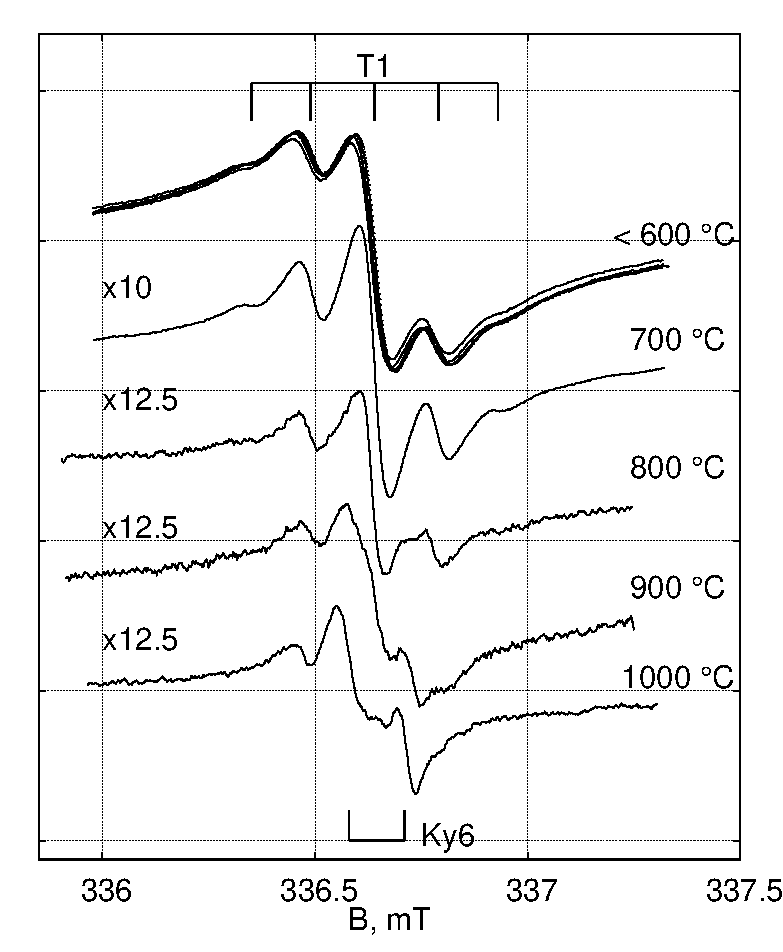
\includegraphics[width=200pt]{images/g1.eps}\mbox{}\\
figure 2\\
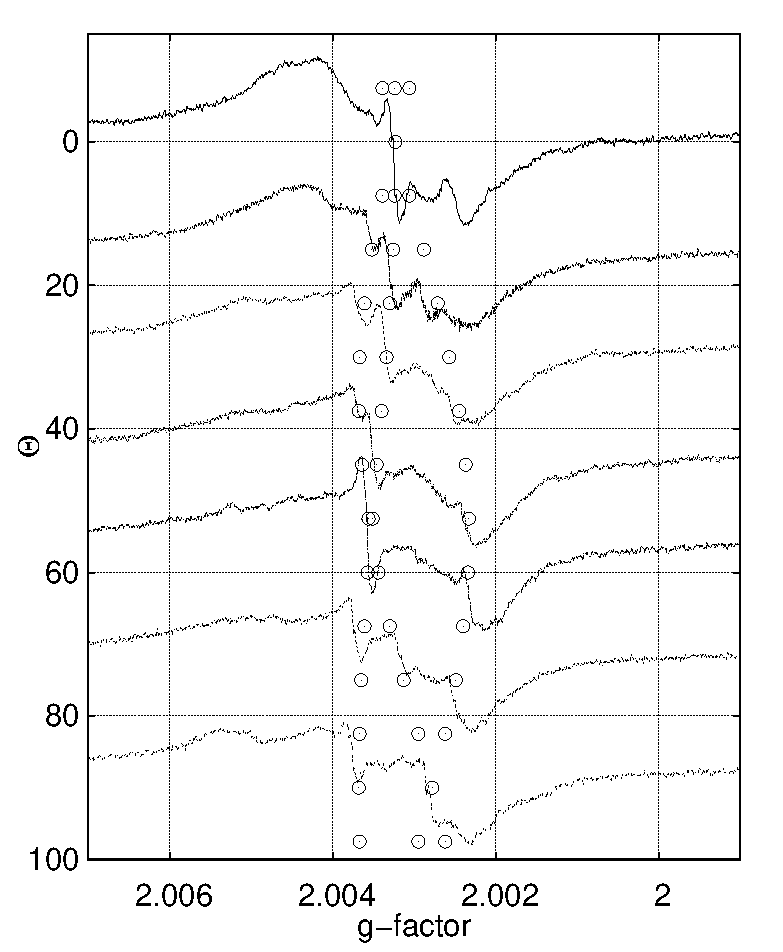
\includegraphics[width=200pt]{images/g2.eps}\mbox{}\\
figure 3\\
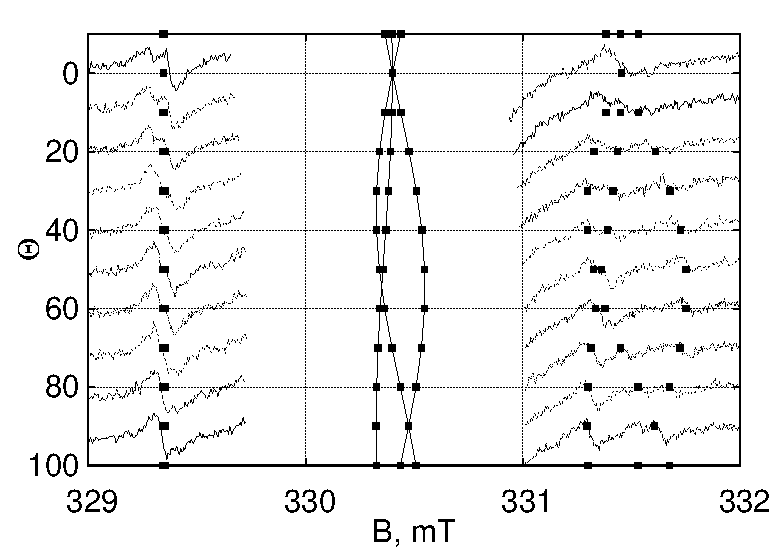
\includegraphics[width=200pt]{images/g3.eps}\mbox{}\\
figure 4\\
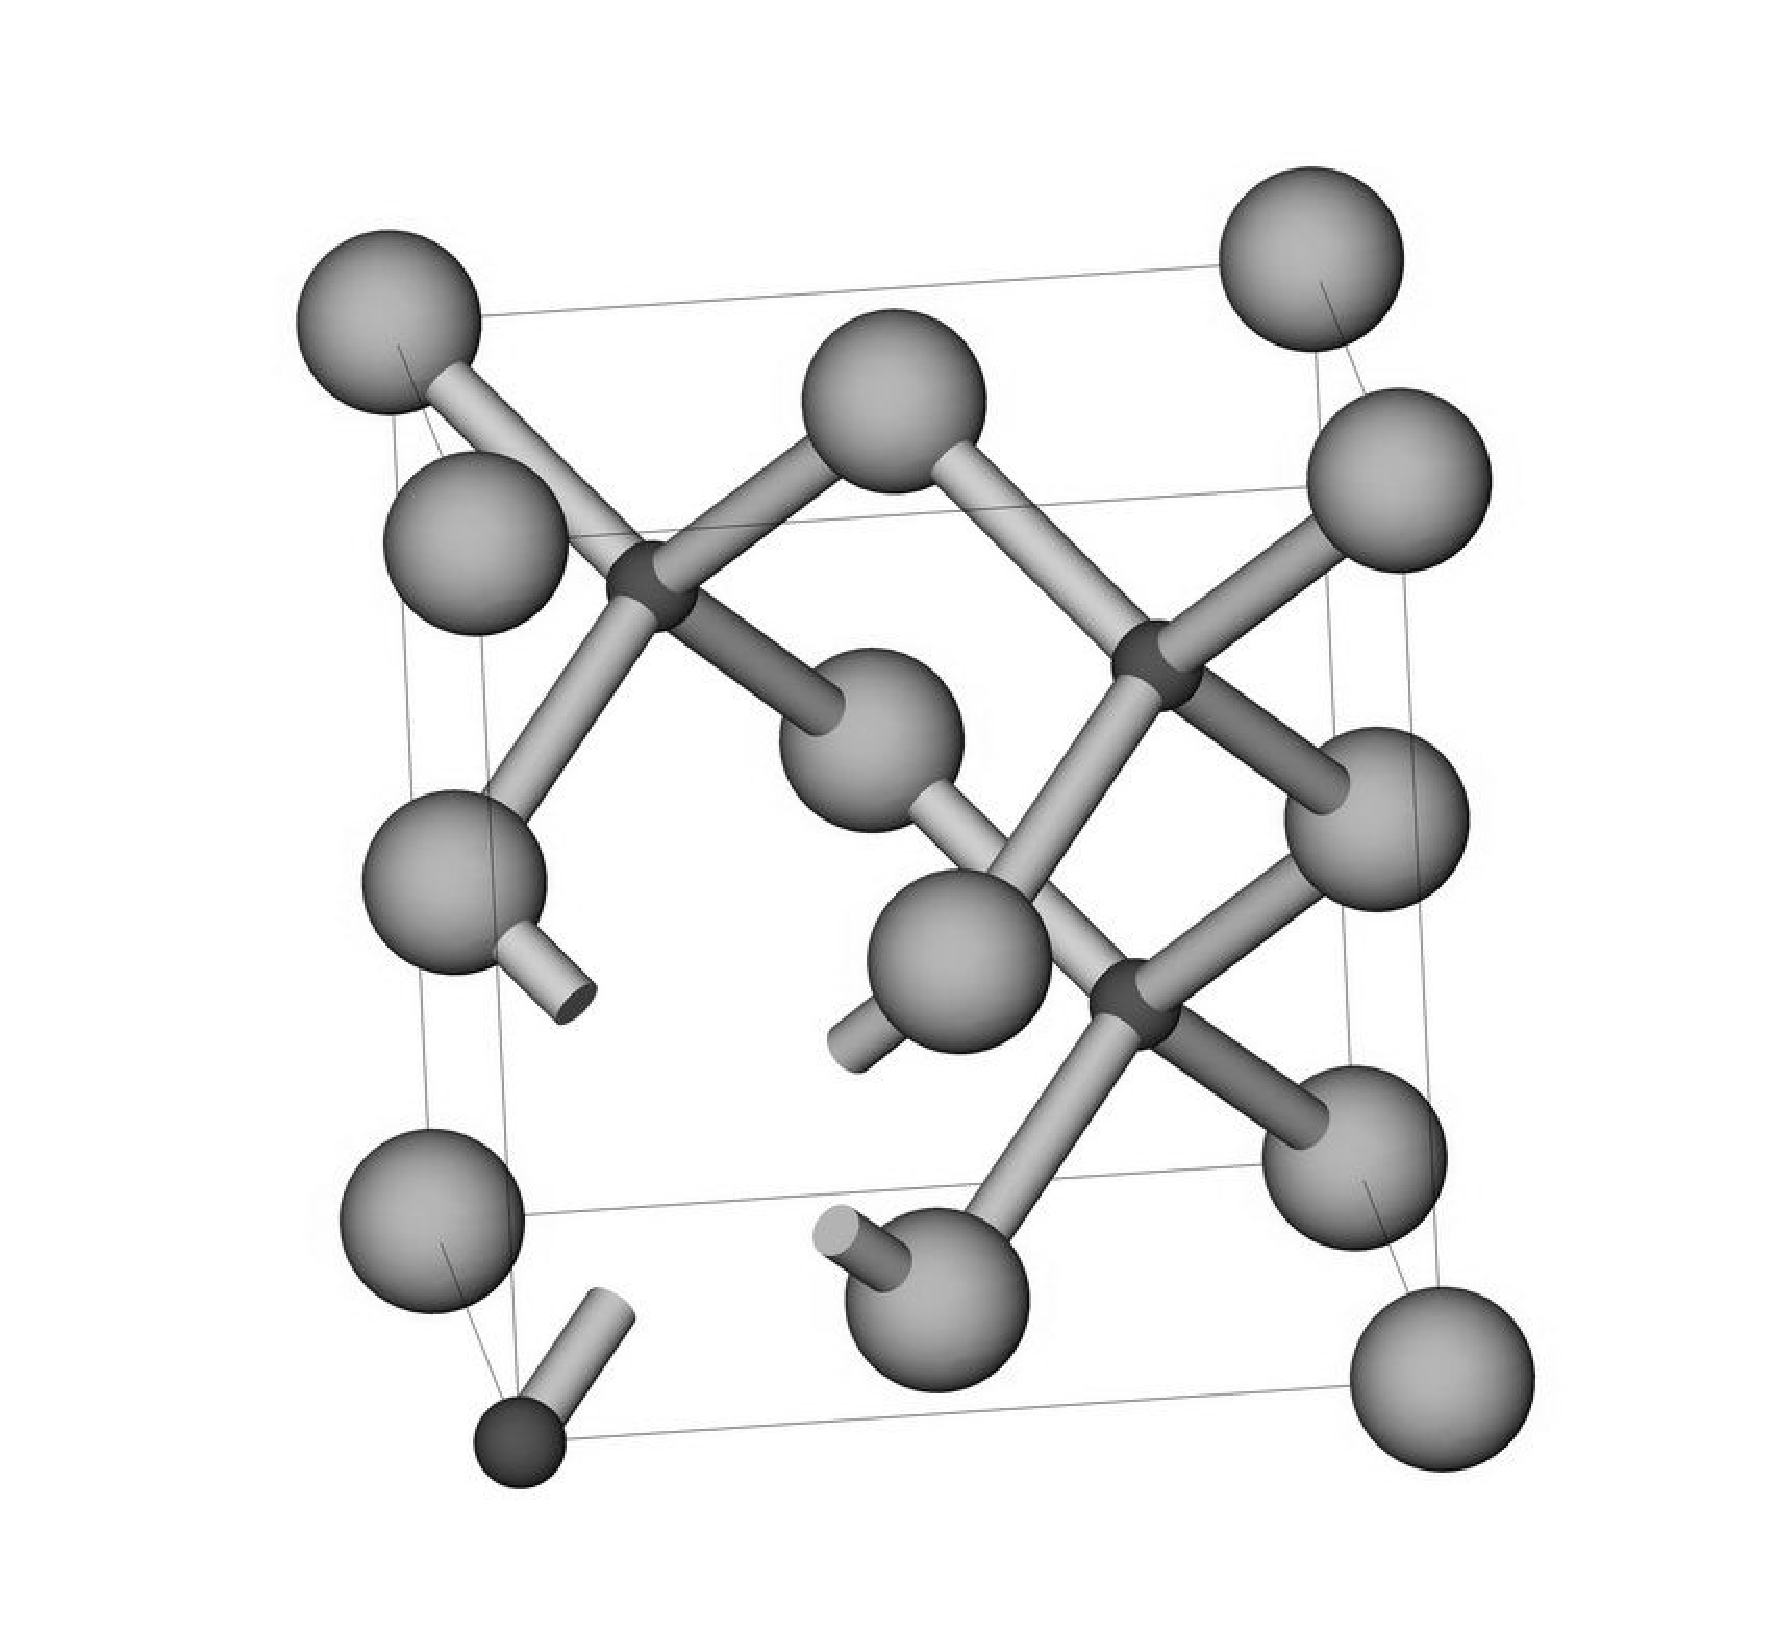
\includegraphics[width=200pt]{images/g4.eps}

%% \label{}

%% The Appendices part is started with the command \appendix;
%% appendix sections are then done as normal sections
%% \appendix

%% \section{}
%% \label{}

%% References
%%
%% Following citation commands can be used in the body text:
%%
%%  \citet{key}  ==>>  Jones et al. (1990)
%%  \citep{key}  ==>>  (Jones et al., 1990)
%%
%% Multiple citations as normal:
%% \citep{key1,key2}         ==>> (Jones et al., 1990; Smith, 1989)
%%                            or  (Jones et al., 1990, 1991)
%%                            or  (Jones et al., 1990a,b)
%% \cite{key} is the equivalent of \citet{key} in author-year mode
%%
%% Full author lists may be forced with \citet* or \citep*, e.g.
%%   \citep*{key}            ==>> (Jones, Baker, and Williams, 1990)
%%
%% Optional notes as:
%%   \citep[chap. 2]{key}    ==>> (Jones et al., 1990, chap. 2)
%%   \citep[e.g.,][]{key}    ==>> (e.g., Jones et al., 1990)
%%   \citep[see][pg. 34]{key}==>> (see Jones et al., 1990, pg. 34)
%%  (Note: in standard LaTeX, only one note is allowed, after the ref.
%%   Here, one note is like the standard, two make pre- and post-notes.)
%%
%%   \citealt{key}          ==>> Jones et al. 1990
%%   \citealt*{key}         ==>> Jones, Baker, and Williams 1990
%%   \citealp{key}          ==>> Jones et al., 1990
%%   \citealp*{key}         ==>> Jones, Baker, and Williams, 1990
%%
%% Additional citation possibilities
%%   \citeauthor{key}       ==>> Jones et al.
%%   \citeauthor*{key}      ==>> Jones, Baker, and Williams
%%   \citeyear{key}         ==>> 1990
%%   \citeyearpar{key}      ==>> (1990)
%%   \citetext{priv. comm.} ==>> (priv. comm.)
%%   \citenum{key}          ==>> 11 [non-superscripted]
%% Note: full author lists depends on whether the bib style supports them;
%%       if not, the abbreviated list is printed even when full requested.
%%
%% For names like della Robbia at the start of a sentence, use
%%   \Citet{dRob98}         ==>> Della Robbia (1998)
%%   \Citep{dRob98}         ==>> (Della Robbia, 1998)
%%   \Citeauthor{dRob98}    ==>> Della Robbia


%% References with bibTeX database:

%% \bibliographystyle{elsarticle-harv}
%% \bibliography{<your-bib-database>}

%% Authors are advised to submit their bibtex database files. They are
%% requested to list a bibtex style file in the manuscript if they do
%% not want to use elsarticle-harv.bst.

%% References without bibTeX database:

\begin{thebibliography}{50}

%% \bibitem must have one of the following forms:
        \bibitem{brun1} F. Bruneval and G. Roma, Phys. Rev. B 83, 144116 (2011)
    \bibitem{choy1} W.J. Choyke, G. Pensl, MRS Bull. No. 3 (1997) 25
    \bibitem{hex1} J. Isoya, T. Umeda, N. Mizuochi, E. Janzen, T. Ohshima, Phys. Status Solidi B 245 (2008) 1298. 
    \bibitem{hex2} N.T. Son, B. Magnusson, Z. Zolnai, A. Ellison, E. Janzen, Mater. Sci. Forum 457-460 (2004) 437.
    \bibitem{epilay} W.J. Choyke, H. Matsunami, G. Pensl (Eds.), Silicon Carbide: Recent Major Advances, 2004, Springer, Berlin, Heidelberg.
    \bibitem{t1} H. Itoh, A. Kawasuso, T. Ohshima, M. Yoshikawa, I. Nashiyama, S. Tanigawa, S. Misawa, H. Okumura, S. Yoshida, Physica Status Solidi A 162 (1997) 173-198.
    \bibitem{ky5} V.Ya. Bratus’, R.S. Melnik, S.M. Okulov, V.N. Rodionov, B.D. Shanina, M.I. Smoliy, Physica B 404 (2009) 4739-4741.
    \bibitem{neut} F. Maekawa, K. Ochiai, K. Shibata, Y. Kasugai, M. Wada, Y. Morimoto, H. Takeuchi, Fusion Eng. Des. 58–59 (2001) 595.


    %\bibitem{brun1} F. Bruneval and G. Roma, Phys. Rev. B 83, 144116 (2011)
%%   \bibitem[Jones et al.(1990)Jones, Baker, and Williams]{key}...
%%   \bibitem[Jones et al., 1990]{key}...
%%   \bibitem[\protect\citeauthoryear{Jones, Baker, and Williams}{Jones
%%       et al.}{1990}]{key}...
%%   \bibitem[\protect\citeauthoryear{Jones et al.}{1990}]{key}...
%%   \bibitem[\protect\astroncite{Jones et al.}{1990}]{key}...
%%   \bibitem[\protect\citename{Jones et al., }1990]{key}...
%%   \harvarditem[Jones et al.]{Jones, Baker, and Williams}{1990}{key}...
%%

% \bibitem[ ()]{}

\end{thebibliography}

\end{document}

%%
%% End of file `elsarticle-template-harv.tex'.
